\chapter{Method}

This chapter describes \ldots compares \ldots


\section{Requirements}

Informed by the findings of research discussed in chapter~\_, some requirements can be specified.





\section{Artoo}

Artoo can be considered to consist of several separate parts:

\begin{description}

\item[{\tt SVGGraph}] A representation of a domain graph -- not necessarily a GSN argument.
This consists of SVG shapes, most of which are graph nodes containing textual labels in the form of SVG {\ttForeignObject}s; and SVG paths representing the graph's directed edges.
The shapes can be moved around the canvas by clicking and dragging, and the edges appear as automatically drawn quadratic B\'{e}zier curves. 

Although this abstraction is described as ''general SVG graph tool code'', many of its features included appear to anticipate GSN-specific use, such as the ability to attach diamonds to shapes (representing undeveloped parts of the argument), the notion of connections being either horizontal (anticipating the GSN's InContextOf relationship) or vertical, and the particular SVG shapes on offer (rectangle, rhomboid, , etc. -- all happen to correspond with types of GSN element).

\item[{\tt GSNGraph}] A wrapper around {\tt SVGGraph}, containing additional methods and [packaging/cloaking/abstracting] it with GSN-specific terminology. 

\end{description}

\section{Experimental methodology}


\subsection{Test data}

\begin{itemize}
    \item Four graphs from \citet{aldenthesis}
\end{itemize}

Up to a point, GSN arguments are quite homogeneous. 


\section{Springy}

Springy.js is an existing JavaScript implementation of a force directed graph drawing algorithm.
It lays out graphs by representing nodes as point charges and edges as springs. Springy.js simulates the electrostatic forces of interaction between these point charges, and the extension of the springs caused by these forces, according to Coulomb's and Hooke's laws.


\subsection{Implementing }

Springy, as distributed [online], consists of a layout algorithm implemented in JavaScript (springy.js) along with a sample renderer for displaying a graph layout.

\section{Arbor}

Simple though the brute-force force directed algorithm implemented in Springy is to understand, it also inefficient.

The Barnes-Hut algorithm is $O$



\section{Dagre}

An key part of the layered layout approach is notion that directed graphs flow in a single direction (typically from top to bottom or from left to right). This is highly applicable to GSN arguments, particularly as specified by the GSN community standard document's guidelines \cite{gsnspec} (see )

Figure~\ref{fig:dagre1} shows

\begin{figure}
  \centering
  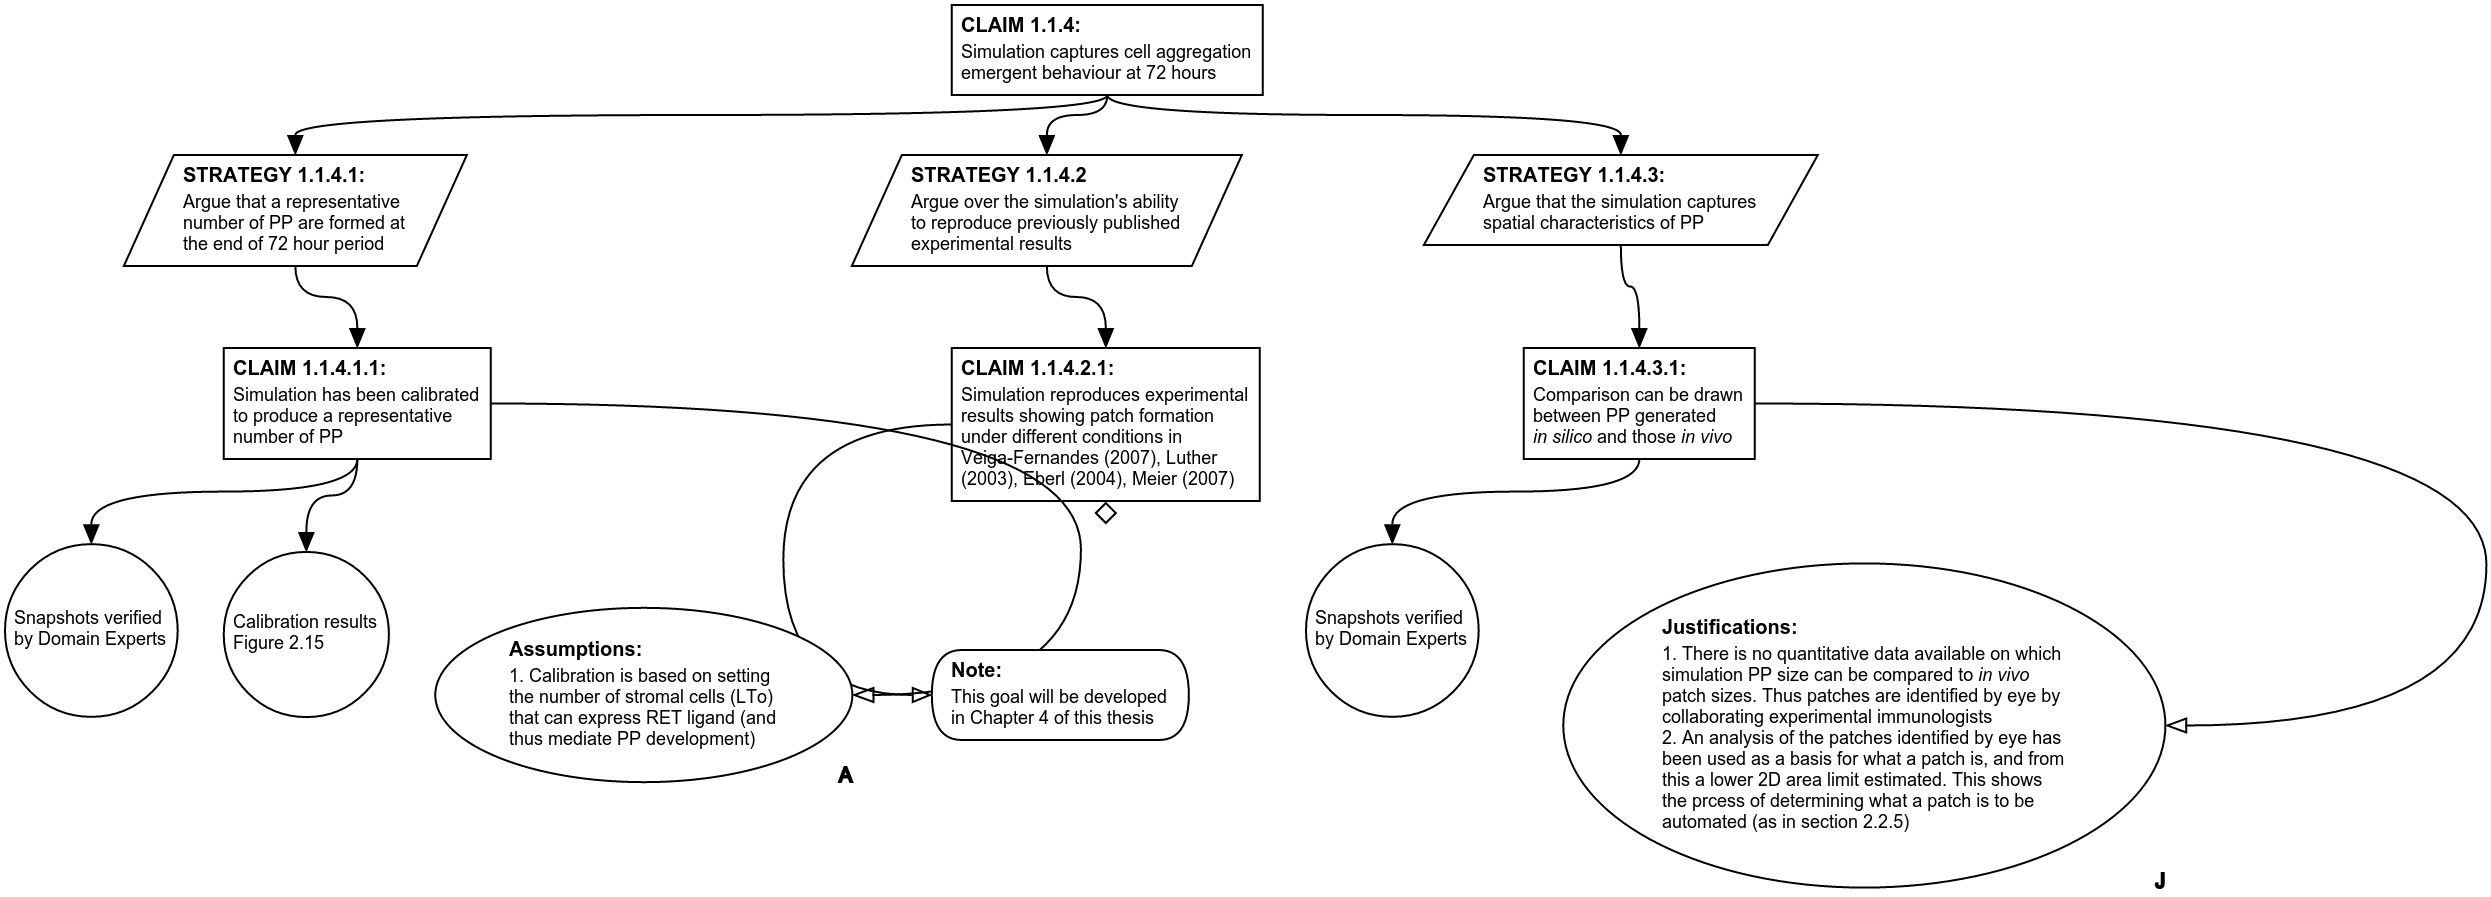
\includegraphics[width=\textwidth]{graphics/results/dagre.png}
  \caption{A na\"ive use of Dagre to render a graph from \cite{aldenthesis}}
  \label{fig:dagre1}
\end{figure}



\begin{figure}
  \centering
  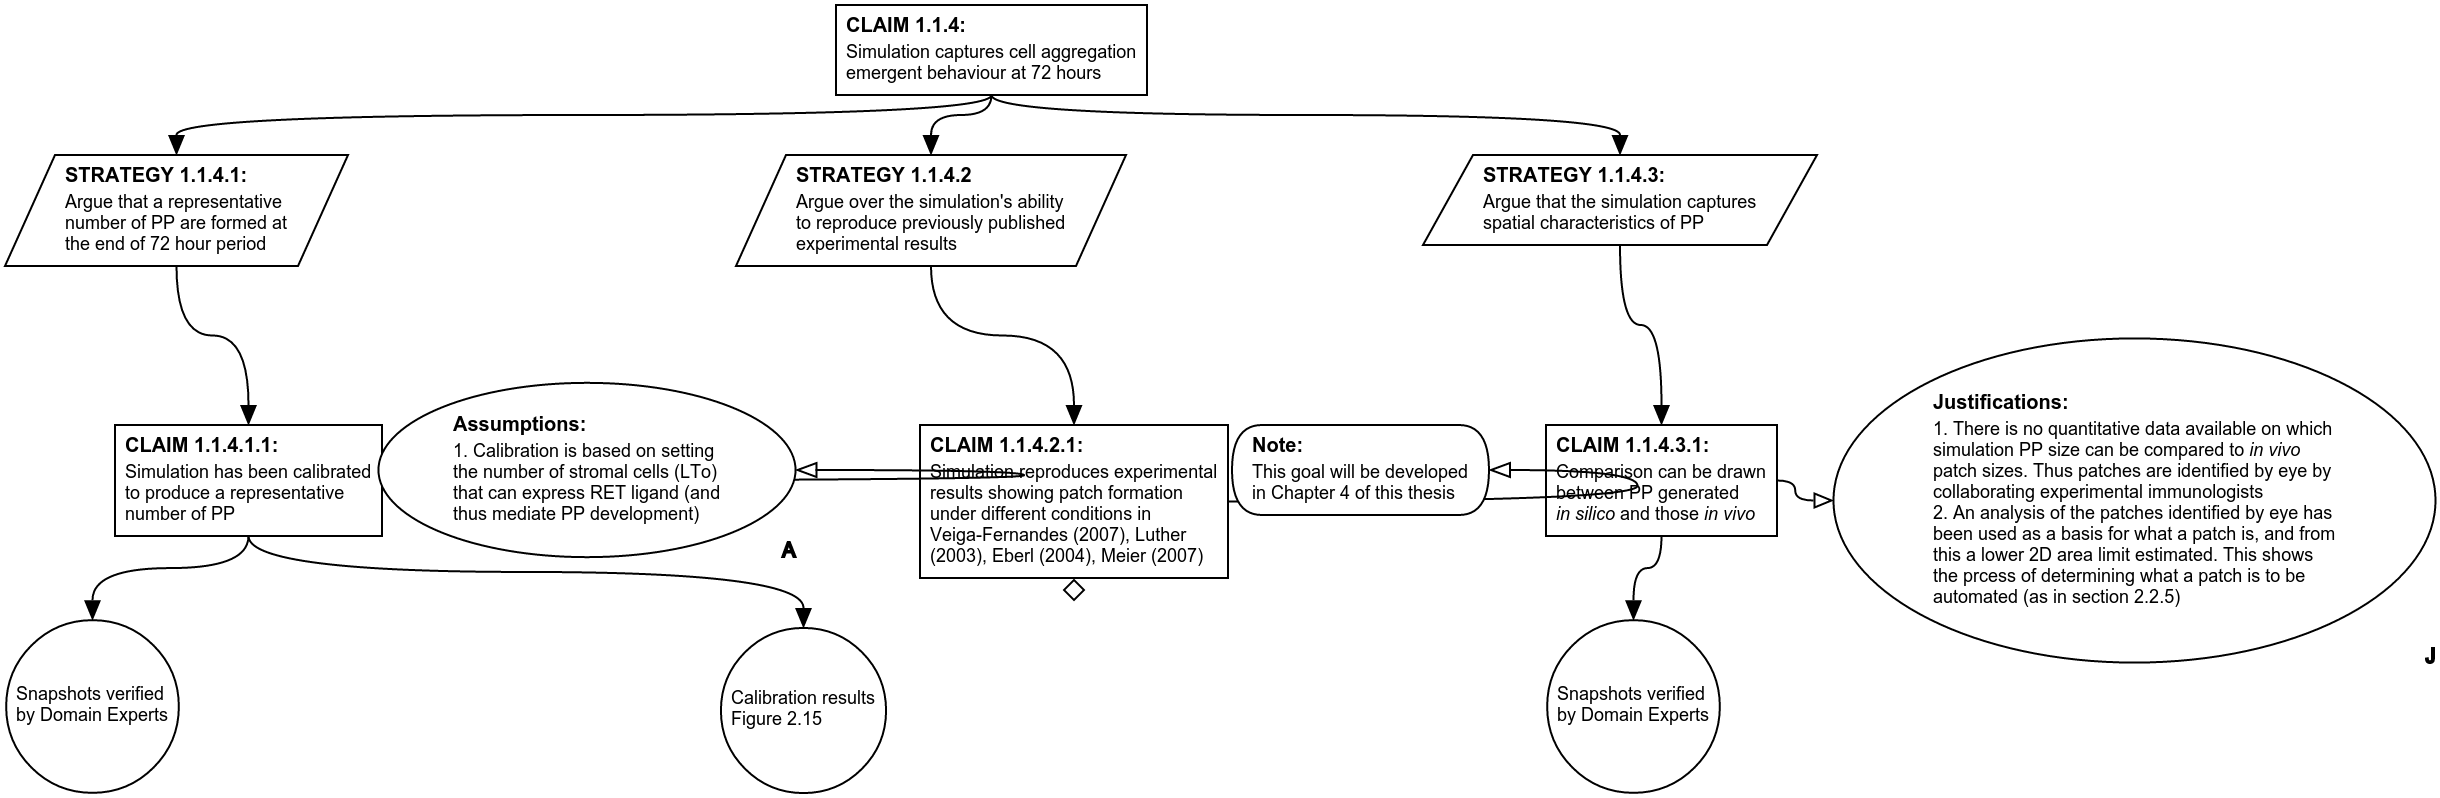
\includegraphics[width=\textwidth]{graphics/results/dagre-enhanced.png}
  \caption{A less na\"ive use of Dagre compared to figure~\ref{fig:dagre}, with context, assumption and justification elements placed to the sides through the use of unrendered dummy elements}
  \label{fig:dagre2}
\end{figure}



\begin{landscape}

\section{Testing}



\subsection{Results}

\subsubsection{Dagre}

\begin{tabular}{ | c | c | c | c | }
    \hline
    Graph & Area & Running time & Edge crossings \\
    \hline
    1     & & & \\
    \hline
    2     & & & \\
    \hline
    3     & & & \\
    \hline
    4     & & & \\
    \hline
\end{tabular}



\end{landscape}
